\section{Exo-alien}


\begin{rpg-commentbox}{Exo-alien}
    The decomposing body of the host is transformed into a liquid cocoon. The parasite uses the host's DNA to fully morph into a powerful insect like alien.  The tendrils on its belly carry spores and the exo-alien playfully leave some of its victims alive so it can reproduce. In the lack of victims, its tendrils touches any possible surface making sure that future parasites will infect whoever dares to explore the den of the beast.

\end{rpg-commentbox}    


\begin{rpg-commentbox}{}

    \centering{\textbf{Stats}}

    \par\noindent\rule{\textwidth}{0.4pt}

    \textbf{SPEED} 2

    \textbf{HEALTH}: 8

    \textbf{SKILLS}: Mobility 5, Observation 8
    
    \textbf{ARMOR}: 12 (5 vs fire)
    
    \textbf{ACID SPLASH}: 8

    \par\noindent\rule{\textwidth}{0.4pt}

    \begin{small}
    \begin{enumerate}
        \item ASSESSING THE THREAT: The exo-Alien pauses, hissing quietly but all the more threatening
        for that. It looks like it’s thinking, 
        or maybe giving silent orders to unseen companions. Everyone within MEDIUM range gets +1 STRESS LEVEL.

        \par\noindent\rule{.9\textwidth}{0.4pt}
        
        \item  ALL-OUT ATTACK: The exo-Alien launches into a wild attack, throwing every one of its tendrils at its victim. It attacks with ten Base Dice, Damage 2. If the victim takes damage, it is infected with a disease with Virulence 6.

        \par\noindent\rule{.9\textwidth}{0.4pt}

        \item BEASTLY BITE: The exo-Alien takes a huge bite from its victim. The attack is rolled with ten
        Base Dice, Damage 1. If the attack causes any damage, it inflicts critical injury \#61 even if
        the victim isn’t Broken, triggering a Panic Roll.
        
        \par\noindent\rule{.9\textwidth}{0.4pt}

        \item CRUSHING BLOW: The exo-Alien brings its entire weight down on the poor victim, who must
        make a MOBILITY roll at –2 (no action) or be crushed, immediately suffering three critical
        injuries (roll three times on the critical injury table and apply all three results, regardless of
        whether or not the victim is Broken). The victim is knocked to the ground and must make
        an immediate Panic Roll

        \par\noindent\rule{.9\textwidth}{0.4pt}

        \item TAIL SPIKE: The tail impales the victim with terrible force. Roll for the attack using ten Base
        Dice (fourteen for a Queen), Damage 1. The attack is armor piercing. If the attack causes
        any damage it automatically triggers critical injury \#66, killing them outright

        \par\noindent\rule{.9\textwidth}{0.4pt}


        \item BELLY TENDRILS: The exo-Alien opens its mouth wide and the inner jaws lash out. The attack uses
        ten Base Dice, Damage 2. If it causes any damage the victim immediately suffers critical
        injury \#64, killing them in one dreadful blow.
    \end{enumerate}
    \end{small}

\end{rpg-commentbox}


\begin{figure}
    \centering
    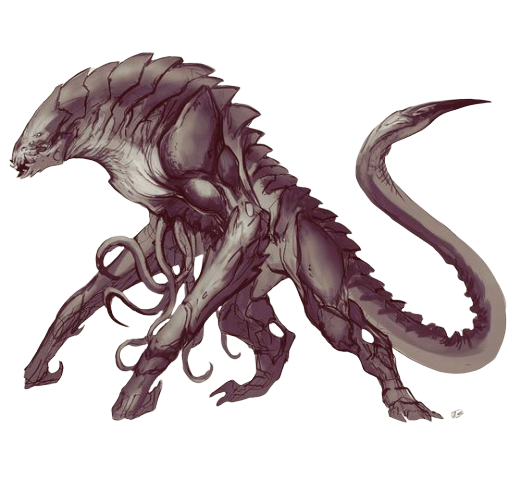
\includegraphics[width=.6\textwidth]{img/stage-III-bg.png}
    \label{fig:stage-3}
    \caption*{Stage III - Exo-alien}
\end{figure}


\section{Exo-Spore}

\begin{rpg-commentbox}{Exo-spore}
    Released by the exo-alien the spore can survive the test of time, below-zero temperatures, and even high-temperatures. If an exo-alien dies of age or from starvation its carapace makes a cocoon that, when under crush pressure, will explode and release spores in a wide area. This is basically what happened in the refinery. A exo-cocoon fossilized within the lithium ore.
\end{rpg-commentbox}